\documentclass[11pt,a4paper]{article}
\usepackage{fontspec}
\setmainfont{TeX Gyre Pagella}
\newfontfamily\headfont{Inter}[UprightFont=*-ExtraBold,BoldFont=*-ExtraBold,Extension=.otf,Path=/usr/share/fonts/opentype/inter/]
\usepackage[a4paper,margin=2.3cm]{geometry}
\usepackage{graphicx,booktabs,float,caption,array,xcolor,longtable}
\usepackage{xurl}
\usepackage[hidelinks]{hyperref}
\usepackage{titlesec}
\usepackage[round]{natbib}
\usepackage{setspace}
\setstretch{1.05}
\renewcommand{\topfraction}{0.9}
\renewcommand{\bottomfraction}{0.8}
\renewcommand{\textfraction}{0.1}
\renewcommand{\floatpagefraction}{0.75}
\setlength{\parindent}{0pt}
\setlength{\parskip}{0.55em}
\titleformat{\section}{\headfont\Large}{\thesection}{0.8em}{}
\titleformat{\subsection}{\headfont\large}{\thesubsection}{0.8em}{}
\captionsetup{font=small,labelfont=bf}
\urlstyle{same}
\hypersetup{pdftitle={How the World Is Governed},pdfauthor={Tristan Hotham}}

\begin{document}
\begin{center}
{\Large\bfseries How the World Is Governed\par}
\vspace{0.4em}
{\large A feature-by-feature classification of 197 systems of government,\\cross-checked against V-Dem and the CIA World Factbook\par}
\vspace{1.2em}
{\large Tristan Hotham\par}
\vspace{0.3em}
{\small Independent researcher\\
ORCID: 0000-0003-4931-9349\\
DOI: https://doi.org/10.5281/zenodo.23863540\par}
\vspace{0.8em}
2026
\end{center}

\begin{quote}
\small
\begin{center}\textbf{Abstract}\end{center}
Maps of political regimes usually sort countries into democracies and autocracies. I classify the constitutional form of all 197 states (the 193 UN members, the Holy See, Palestine, Taiwan and Kosovo) on eight features: the kind of head of state, how that office is filled, the executive type (including the premier-presidential and president-parliamentary subtypes of semi-presidentialism), whether head of state and head of government are one office, the territorial structure, the number of chambers, the electoral system of the lower or only chamber and any power sharing fixed by community. Each field is derived by stated rules from two independent sources, V-Dem v16 (latest year 2025) and the CIA World Factbook (2026 and 2024 editions), compared cell by cell, with 83 documented and cited hand decisions. The countries fall into 12 families and 112 exact systems, of which 80 belong to a single country; those 80 countries hold 42\% of the world's population. The largest shared system, unitary parliamentary republics with one chamber elected by list proportional representation, has 14 members. Presidential republics (52) and parliamentary republics (45) are the largest families and each holds over a quarter of humanity; 25 federations hold 41\%. Set against V-Dem's Regimes of the World, 71\% of countries electing their lower house by proportional representation are democracies against 43\% of majoritarian ones, 78\% of premier-presidential against 11\% of president-parliamentary systems, and ceremonial monarchies have the highest mean Liberal Democracy Index of any family (0.64). These patterns are descriptive. The classification, sources and decisions are released as open data.

\textbf{Keywords:} political systems; forms of government; semi-presidentialism; federalism; electoral systems; V-Dem; Regimes of the World; CIA World Factbook; comparative politics; open data
\end{quote}

\section{Introduction}
The most widely used maps of political systems answer one question: is a country democratic? V-Dem's Regimes of the World \citep{row}, Freedom House and the Economist Intelligence Unit each give two to four classes. They are indispensable, but they describe the quality of a regime rather than its architecture. Two parliamentary republics with ceremonial presidents, Germany and Italy, sit in the same class on such a map, yet Germany is a federation whose Bundestag is elected by mixed-member proportional representation, while Italy is a regionalised state whose Chamber of Deputies is elected by a parallel system. Political scientists have long distinguished these features \citep{lijphart,shugartcarey,elgie2011,reynolds}; open, current, global datasets that put them together for every country are rarer.

This paper builds one. It classifies all 197 states on eight features of constitutional form and practice, derives each field by stated rules from two independent sources, records where they disagree, and documents every hand decision with a citation. It then groups identical combinations (``signatures'') into a hierarchy of families and exact systems, counts how widely each is shared and how many people live under it, and sets the classification beside V-Dem's democracy measures. An interactive version is at \url{https://maps.tristanhotham.com/government-types/}.

\section{Data}
\textbf{V-Dem.} The V-Dem Country-Year Dataset v16 \citep{vdem}, as packaged in the vdemdata R package 16.0 \citep{vdemdata}, latest year 2025, licensed CC BY-SA 4.0 (as listed in the Swedish National Data Service catalogue, \url{https://researchdata.se/en/catalogue/dataset/ext0309-1}). I use the Regimes of the World classification (v2x\_regime), the Liberal and Electoral Democracy Indices (v2x\_libdem, v2x\_polyarchy) with their intervals, and institutional indicators: how the head of state reached office (v2expathhs), whether head of state and head of government are the same (v2exhoshog), the head of state's relative power over the cabinet (v2ex\_hosw), whether the head of state could remove the head of government in practice (v2exrmhgnp\_5), the hereditary, military and party dimensions of the executive's power base, the number of chambers (v2lgbicam), the share of the lower chamber directly elected (v2lgello) and the thirteen-category electoral system of the latest election to the lower chamber (v2elloelsy). V-Dem covers 175 of the 197 states; the 22 not covered are microstates and small island states.

\textbf{CIA World Factbook.} The Factbook as JSON \citep{factbook}, at the repository's final 2026 state and at commit 379131b4 (December 2024), the last snapshot with full-text descriptions of each legislature. The Factbook is a US government work in the public domain. I use its government type, executive branch (chief of state, head of government, election process), legislative structure and electoral system, administrative divisions, and international organisation membership (to define the set of UN member states).

\textbf{Population and boundaries.} World Bank total population for 2025 \citep{wb}, with Natural Earth estimates for Taiwan and the Holy See; Natural Earth 1:50m and 1:10m countries \citep{naturalearth}.

Wikidata and Wikipedia's lists of countries by system of government and by electoral system would make a natural third source; they could not be retrieved for this version and are not used.

\section{Methods}
\subsection{Fields and rules}
\textbf{Head of state.} A country is a monarchy if V-Dem codes its head of state as having reached office by hereditary succession, a royal council or appointment by a foreign power (the Commonwealth realms), or, for countries outside V-Dem, if the Factbook calls it one. A monarchy is \emph{absolute} if the Factbook says so; \emph{constitutional with a ruling monarch} (dualist) if V-Dem codes the head of state as at least as powerful as the head of government over the cabinet (v2ex\_hosw~$\geq$~0.5) or the hereditary dimension as at least 0.5; otherwise \emph{ceremonial}. The office is recorded as hereditary, elective, a monarch abroad or co-princes for monarchies, and as a president, a collective presidency or a Supreme Leader for republics.

\textbf{Executive.} Military government (a head of state who took power by force or was appointed by the military, with a military power base of at least 0.5), one-party state (Factbook ``communist'' or a head of state appointed by the ruling party) and the theocratic and transitional cases (Factbook labels, hand decisions) are assigned first. Monarchies take the executive implied by the monarch's power. For republics, a directly elected president who is also head of government is \emph{presidential}; a head of state who is also head of government but chosen by or through the legislature gives a \emph{parliamentary system with an executive president}, Switzerland's collegial Federal Council a \emph{directorial} system; a head of state not directly elected, with a separate head of government, is \emph{parliamentary}. A directly elected president with a separate prime minister is \emph{semi-presidential} if the Factbook calls the system presidential or semi-presidential or V-Dem codes the president as at least as powerful as the prime minister; otherwise parliamentary. Following \citet{shugartcarey}, semi-presidential systems are \emph{president-parliamentary} where the president can also remove the prime minister (V-Dem v2exrmhgnp\_5 above 0.5) and \emph{premier-presidential} otherwise; France and Ukraine are set by their constitutions, which give the president no such power, although V-Dem's in-practice coding differs.

\textbf{Territory, chambers, elections and power sharing.} Federations are those the Factbook calls federal, plus Argentina and Bosnia and Herzegovina; Italy, Spain and the United Kingdom are \emph{regionalised}; \emph{unitary with autonomous regions} comes from autonomous units in the Factbook's administrative divisions with hand additions and exclusions. Chambers are V-Dem's count of sitting chambers (``none sitting'' where a legislature is dissolved or suspended), checked against the Factbook. The electoral system is V-Dem's code for the latest election, checked against the Factbook's 2026 category and a parse of its 2024 text; a chamber less than half directly elected is ``indirect or appointed''. Power sharing is coded only where the constitution or a binding pact allocates top offices or seats by community (Lebanon, Bosnia and Herzegovina, Belgium, Burundi).

\textbf{Precedence and cross-checks.} For each field a hand decision overrides the rule, V-Dem's in-practice coding is preferred to the Factbook where both exist, and the Factbook is used alone where V-Dem is silent. Each country and field cell records its source values and whether the sources agree, disagree, or only one speaks.

\subsection{Families and signatures}
A country's \emph{signature} is the combination of its eight fields. Identical signatures form an \emph{exact system}. \emph{Families} group countries by head of state and executive into 12 classes; \emph{sub-families} split each family by the broad class of electoral system (majoritarian, mixed or semi-proportional, proportional, not directly elected), giving 39 sub-families. All statistics are descriptive counts and population shares, with population weights from 2025.

\section{Results}
\subsection{Families}
Table~\ref{tab:families} and Figures~\ref{fig:map} and~\ref{fig:families} summarise the families. Presidential republics (52 countries, 27\% of the world's population) and parliamentary republics (45, 28\%) are the largest, followed by 29 parliamentary monarchies (6\%), 14 of them Commonwealth realms. Semi-presidential systems number 27: 18 president-parliamentary, holding 8\% of the world's people, and 9 premier-presidential (2\%). One-party states are only 6 but hold 19\% of humanity. In all, 30 countries with 28\% of the world's people are governed by a party, the military, clerics, a royal family or a transitional authority. There are 43 monarchies (8\% of the population) and 25 federations (41\%).

\begin{table}[tbp]\centering\small\caption{The twelve families: countries, share of world population, exact systems, one-country systems and mean V-Dem Liberal Democracy Index (countries covered by V-Dem).}\label{tab:families}\begin{tabular}{lrrrrr}\toprule Family & Countries & Population & Systems & Unique & Mean LDI\\\midrule
Parliamentary monarchies & 29 & 6.3\% & 20 & 16 & 0.64\\
Ruling monarchies & 7 & 0.7\% & 7 & 7 & 0.18\\
Absolute monarchies & 6 & 0.7\% & 5 & 4 & 0.09\\
Parliamentary republics & 45 & 27.6\% & 22 & 17 & 0.50\\
Assembly-chosen executives & 7 & 1.0\% & 6 & 5 & 0.59\\
Semi-presidential, premier-presidential & 9 & 1.9\% & 6 & 3 & 0.50\\
Semi-presidential, president-parliamentary & 18 & 7.8\% & 9 & 5 & 0.17\\
Presidential republics & 52 & 27.2\% & 20 & 10 & 0.38\\
One-party states & 6 & 19.0\% & 4 & 3 & 0.06\\
Military governments & 8 & 2.9\% & 4 & 2 & 0.11\\
Theocracies & 3 & 1.7\% & 3 & 3 & 0.06\\
Transitional or divided authority & 7 & 3.4\% & 6 & 5 & 0.08\\
\bottomrule\end{tabular}\end{table}

\begin{figure}[tbp]\centering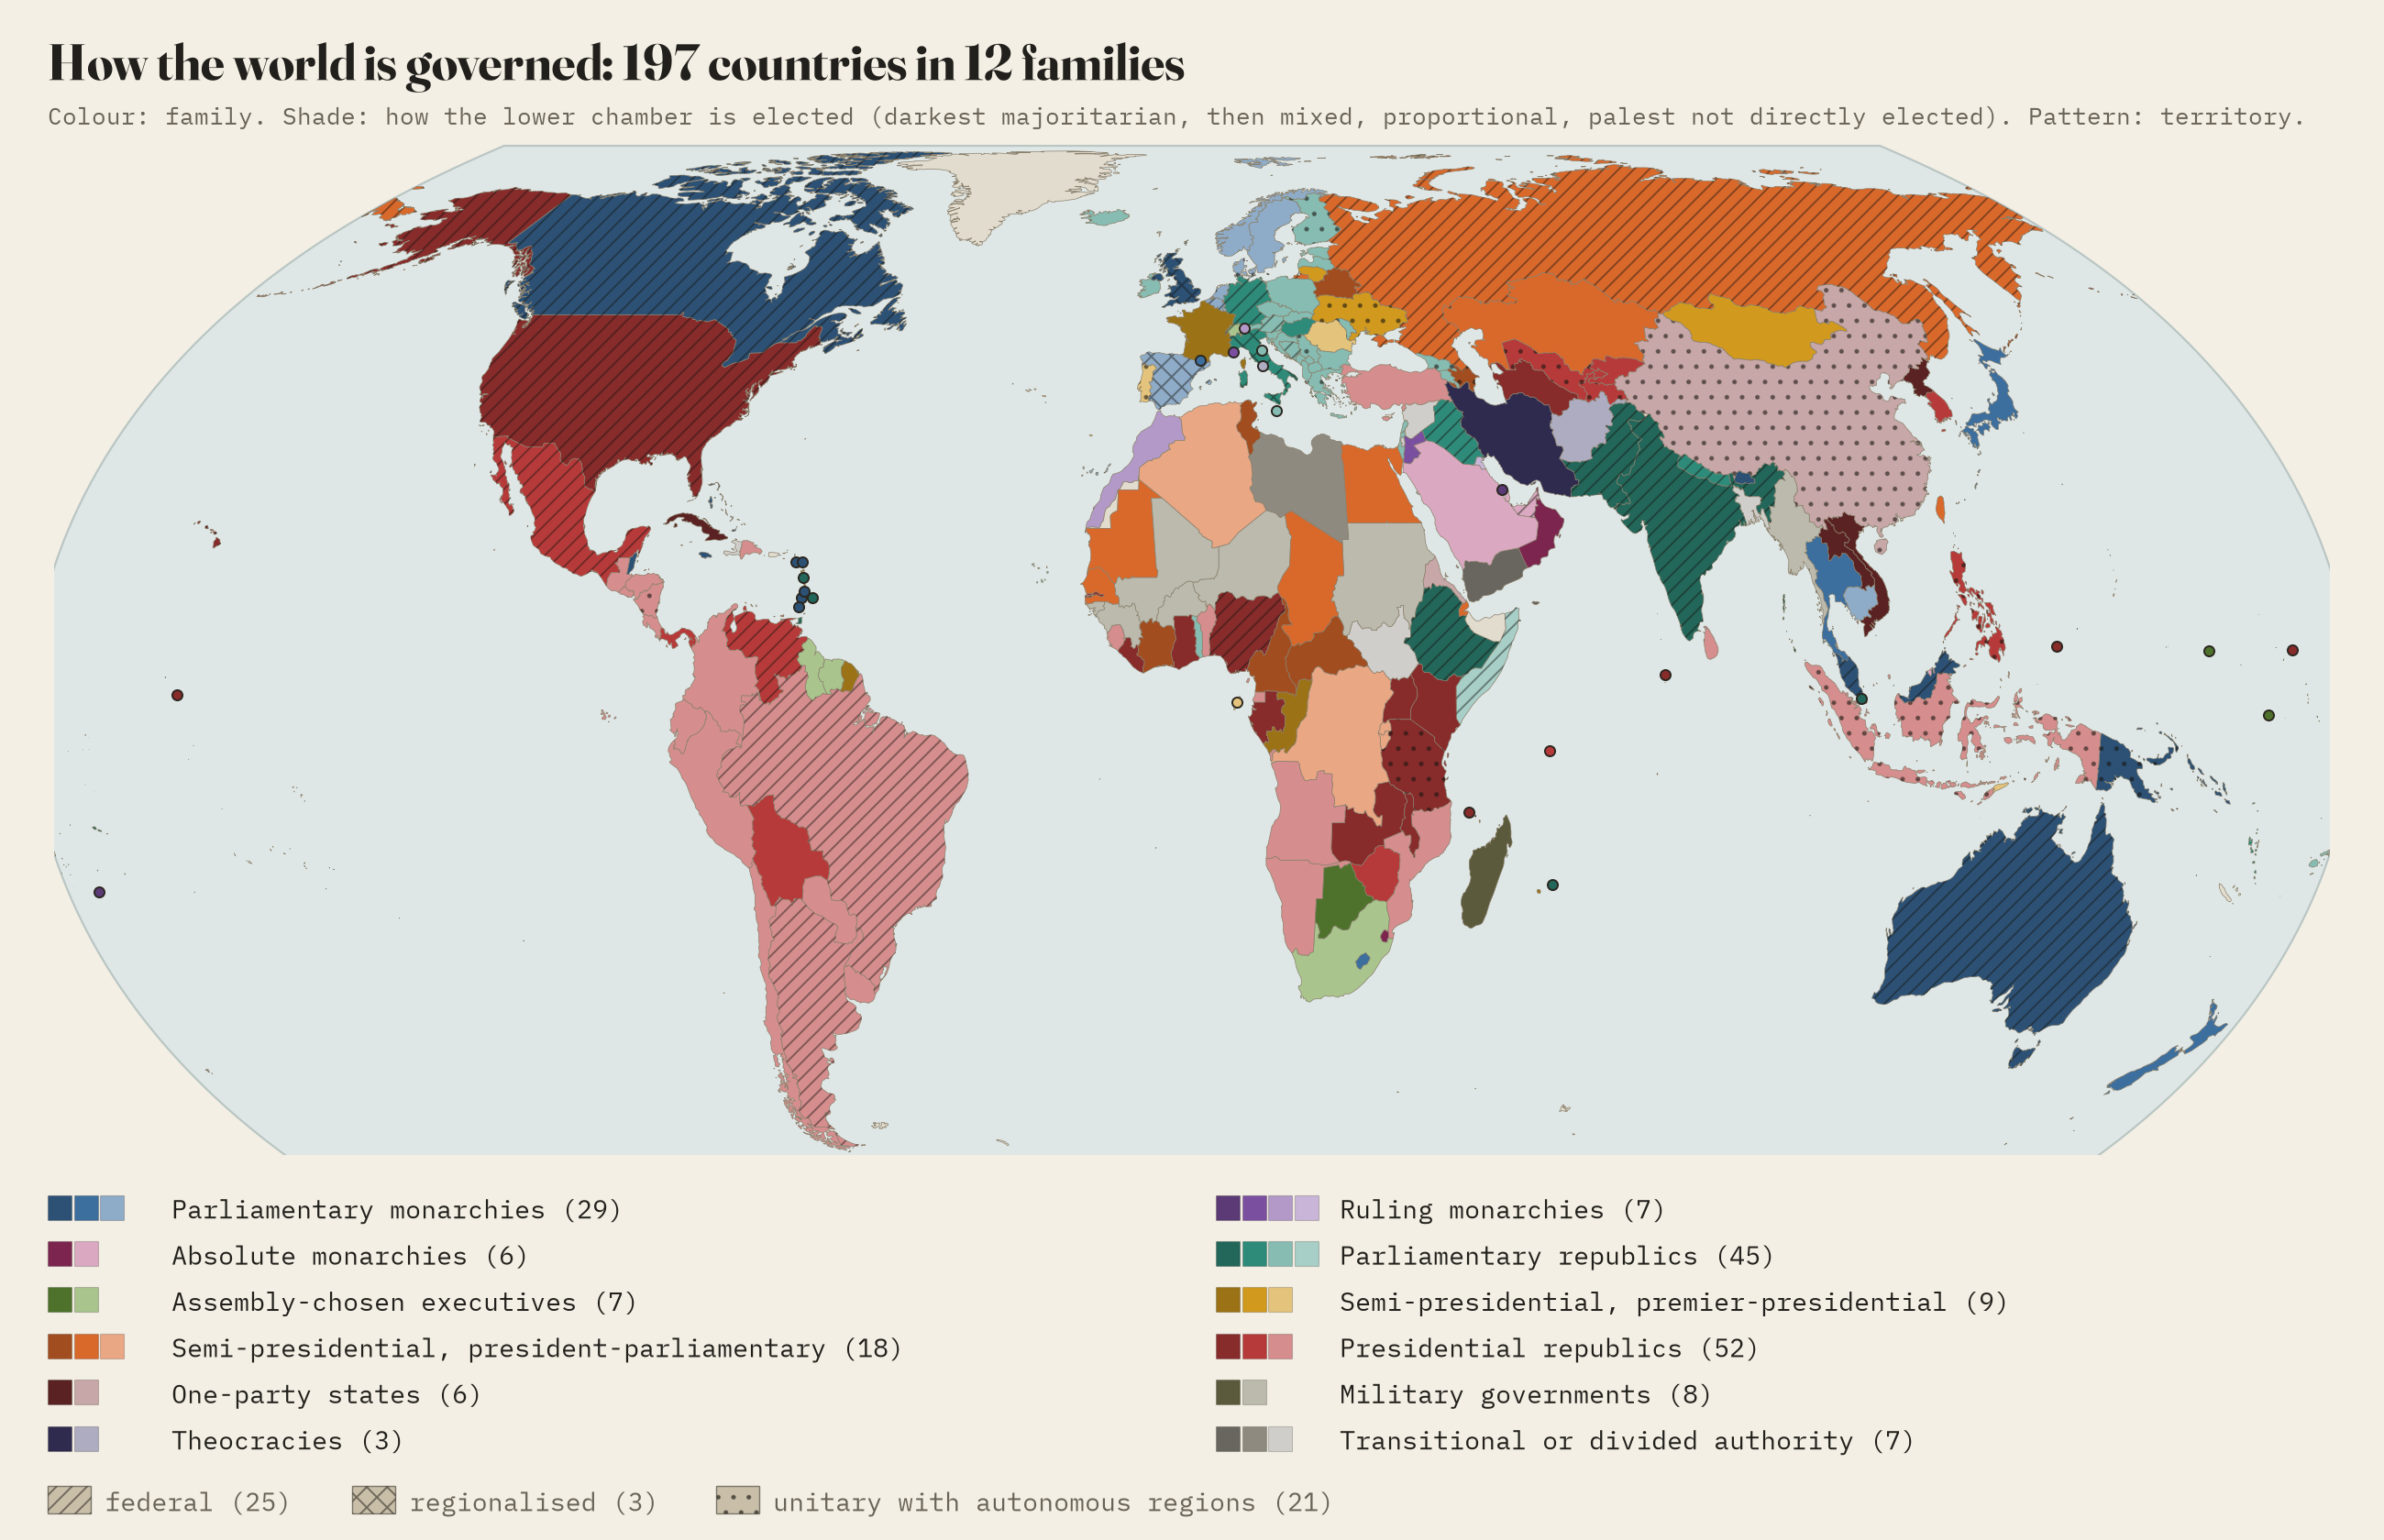
\includegraphics[width=\textwidth]{f_map_family.png}
\caption{Families of government, shaded by the electoral system of the lower or only chamber, with patterns for federal, regionalised and autonomous-region states (Equal Earth projection).}\label{fig:map}\end{figure}

\begin{figure}[tbp]\centering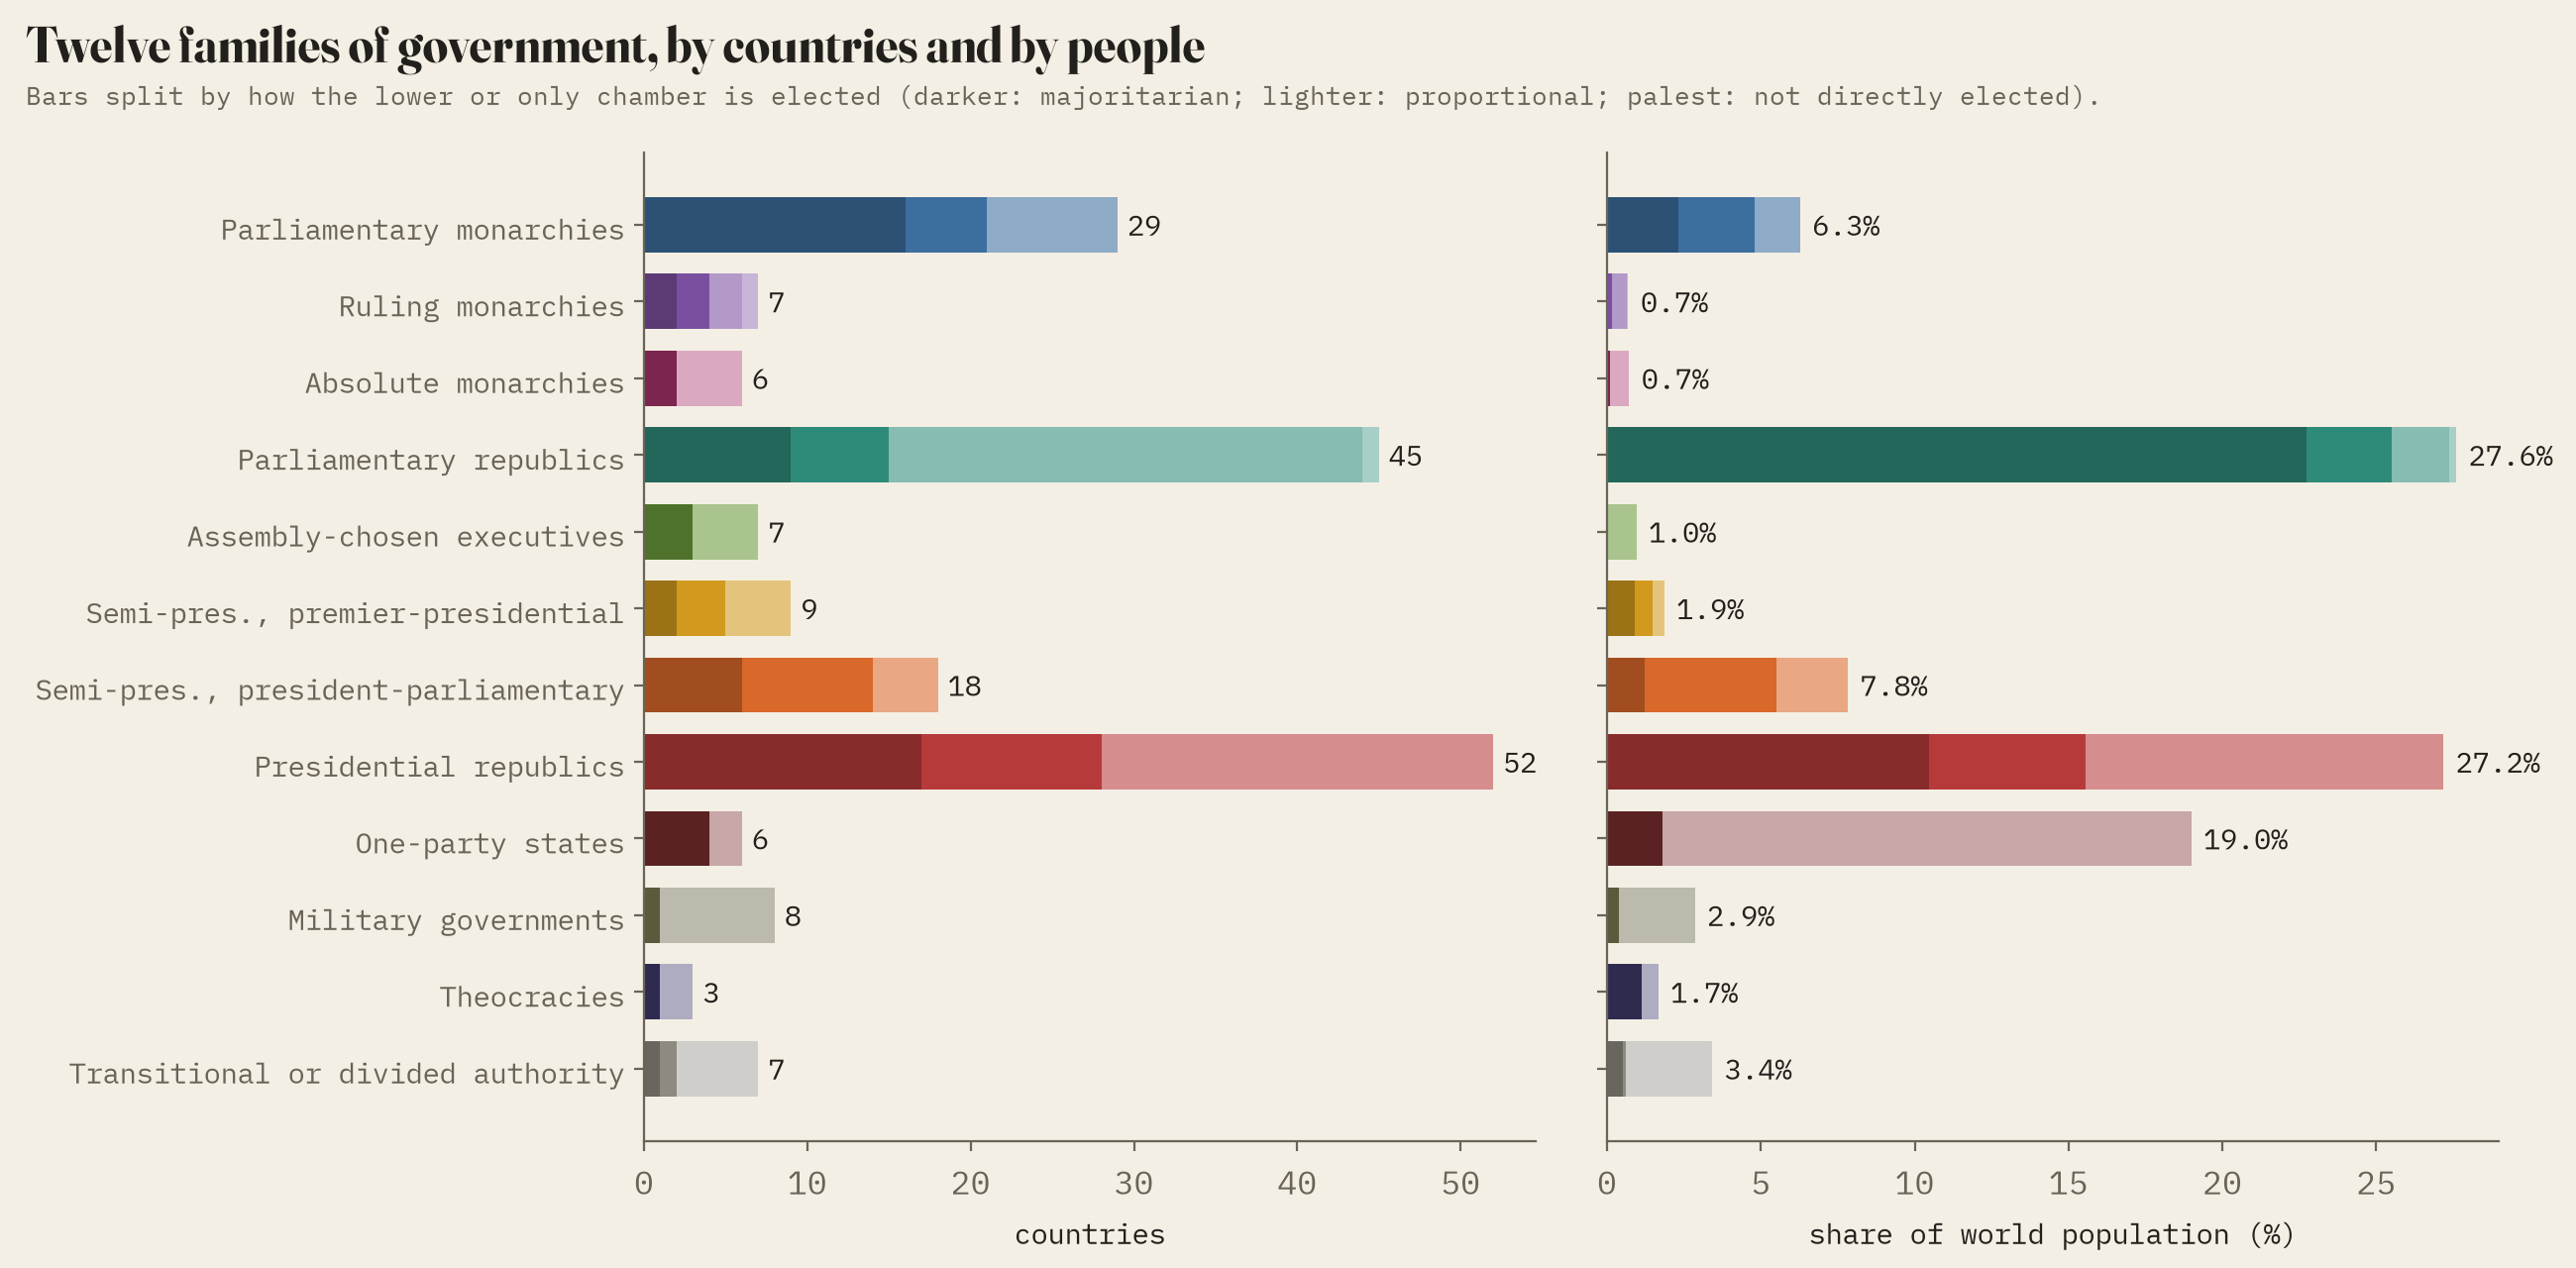
\includegraphics[width=\textwidth]{f_families.png}
\caption{Countries and share of world population in each family, split by electoral system.}\label{fig:families}\end{figure}

\subsection{Exact systems}
The 197 countries have 112 distinct signatures. 32 are shared by two or more countries (117 countries in all) and 80 are unique (Figure~\ref{fig:sigs}, Table~\ref{tab:sigs}). The largest shared system has 14 members, mostly in central and eastern Europe; the second, its presidential counterpart, has 13. India, Pakistan and Ethiopia share an exact system, as do the United States and Nigeria and Brazil and Argentina. Germany and Italy differ in territory and electoral system. France and the Republic of the Congo share an exact system although V-Dem scores their liberal democracy at 0.80 and 0.12. The unique systems include the most populous states with idiosyncratic designs (China, Indonesia, Russia, Mexico, Japan, Iran, Germany) and the textbook one-offs: Switzerland's directorial Federal Council, Bosnia's three-member presidency, Lebanon's confessional parliament, Andorra's co-princes and the Holy See. Without the power-sharing field, Lebanon would share its signature with Israel.

\begin{table}[tbp]\centering\footnotesize\caption{The ten most widely shared exact systems.}\label{tab:sigs}\begin{tabular}{lrp{5.0cm}p{6.6cm}}\toprule System & N & Features & Countries\\\midrule
S001 & 14 & \raggedright Republic; Parliamentary; Unitary; Unicameral; List PR & \raggedright\arraybackslash Albania, Armenia, Bulgaria, Cabo Verde, Croatia, Estonia, Fiji, Iceland, Israel, Kosovo, Latvia, Montenegro, North Macedonia, Slovakia\\
S002 & 13 & \raggedright Republic; Presidential; Unitary; Unicameral; List PR & \raggedright\arraybackslash Angola, Benin, Costa Rica, Cyprus, Ecuador, El Salvador, Guatemala, Honduras, Mozambique, Peru, Sierra Leone, Sri Lanka, Turkey\\
S003 & 7 & \raggedright Republic; Presidential; Unitary; Bicameral; List PR & \raggedright\arraybackslash Chile, Colombia, Dominican Republic, Equatorial Guinea, Namibia, Paraguay, Uruguay\\
S005 & 6 & \raggedright Republic; Presidential; Unitary; Unicameral; FPTP & \raggedright\arraybackslash Gambia, Ghana, Malawi, Maldives, Uganda, Zambia\\
S004 & 6 & \raggedright Ceremonial monarchy; Parliamentary; Unitary; Bicameral; FPTP & \raggedright\arraybackslash Antigua and Barbuda, Bahamas, Belize, Grenada, Jamaica, Saint Lucia\\
S006 & 5 & \raggedright Republic; Parliamentary; Unitary, auton. regions; Unicameral; List PR & \raggedright\arraybackslash Finland, Georgia, Greece, Moldova, Serbia\\
S007 & 4 & \raggedright Republic; Military government; Unitary; Unicameral; Indirect/appointed & \raggedright\arraybackslash Burkina Faso, Guinea, Mali, Niger\\
S009 & 4 & \raggedright Republic; Semi-pres. (pres.-parl.); Unitary; Bicameral; Two-round & \raggedright\arraybackslash Belarus, Cameroon, Côte d'Ivoire, Tunisia\\
S008 & 4 & \raggedright Republic; Parliamentary; Unitary; Bicameral; List PR & \raggedright\arraybackslash Czechia, Poland, Slovenia, Togo\\
S012 & 3 & \raggedright Republic; Parliamentary; Federal; Bicameral; FPTP & \raggedright\arraybackslash Ethiopia, India, Pakistan\\
\bottomrule\end{tabular}\end{table}

\begin{figure}[tbp]\centering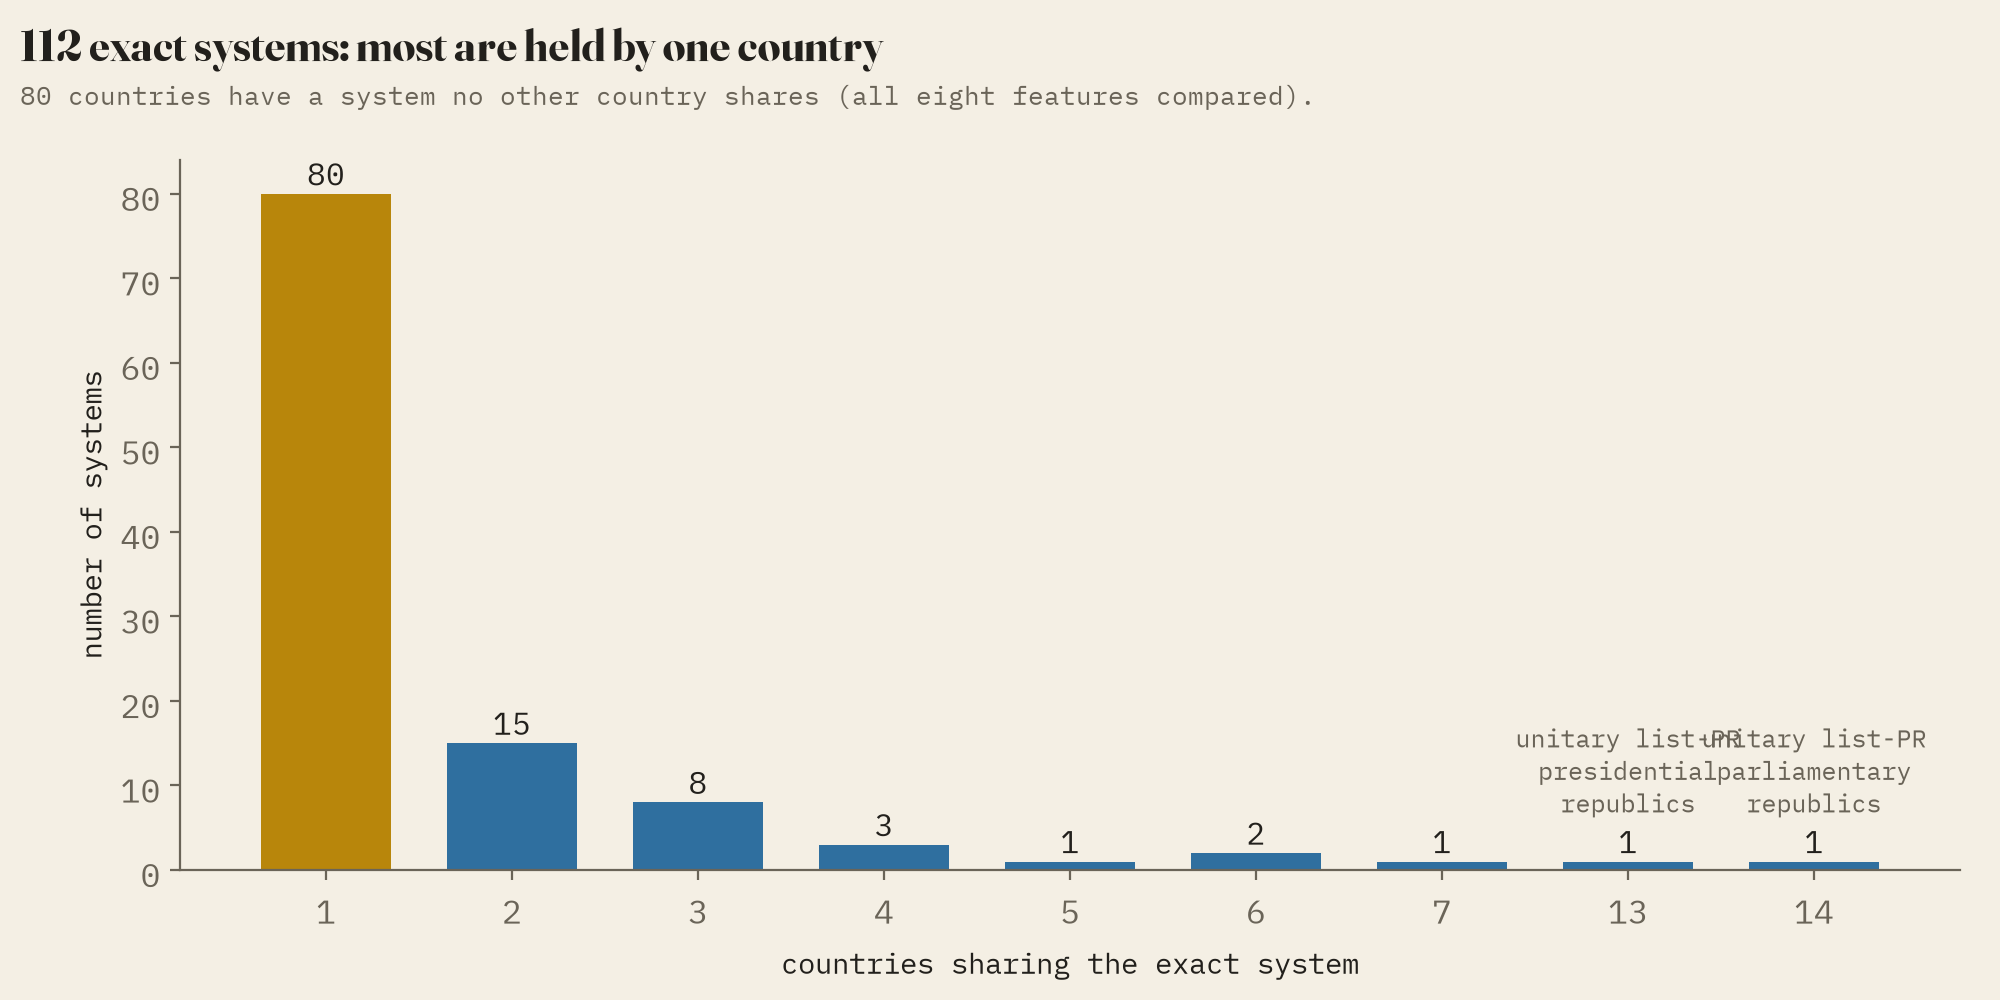
\includegraphics[width=.86\textwidth]{f_signatures.png}
\caption{How many countries share each exact system.}\label{fig:sigs}\end{figure}


\subsection{Single features}
List proportional representation is the commonest electoral system for the lower or only chamber (73 countries) but covers only 19\% of the world's people; first past the post is used by 38 countries with 36\%, 62\% of them in India and the United States (Figure~\ref{fig:elmap}). Mixed systems are used by 34 countries (24 parallel, 10 mixed-member proportional). 22 countries, with 24\% of the world's people, have no directly elected lower chamber or none sitting. 81 legislatures are bicameral, 107 unicameral, and 9 countries have no sitting legislature. In 64 countries one person or body is both head of state and head of government.

\begin{figure}[tbp]\centering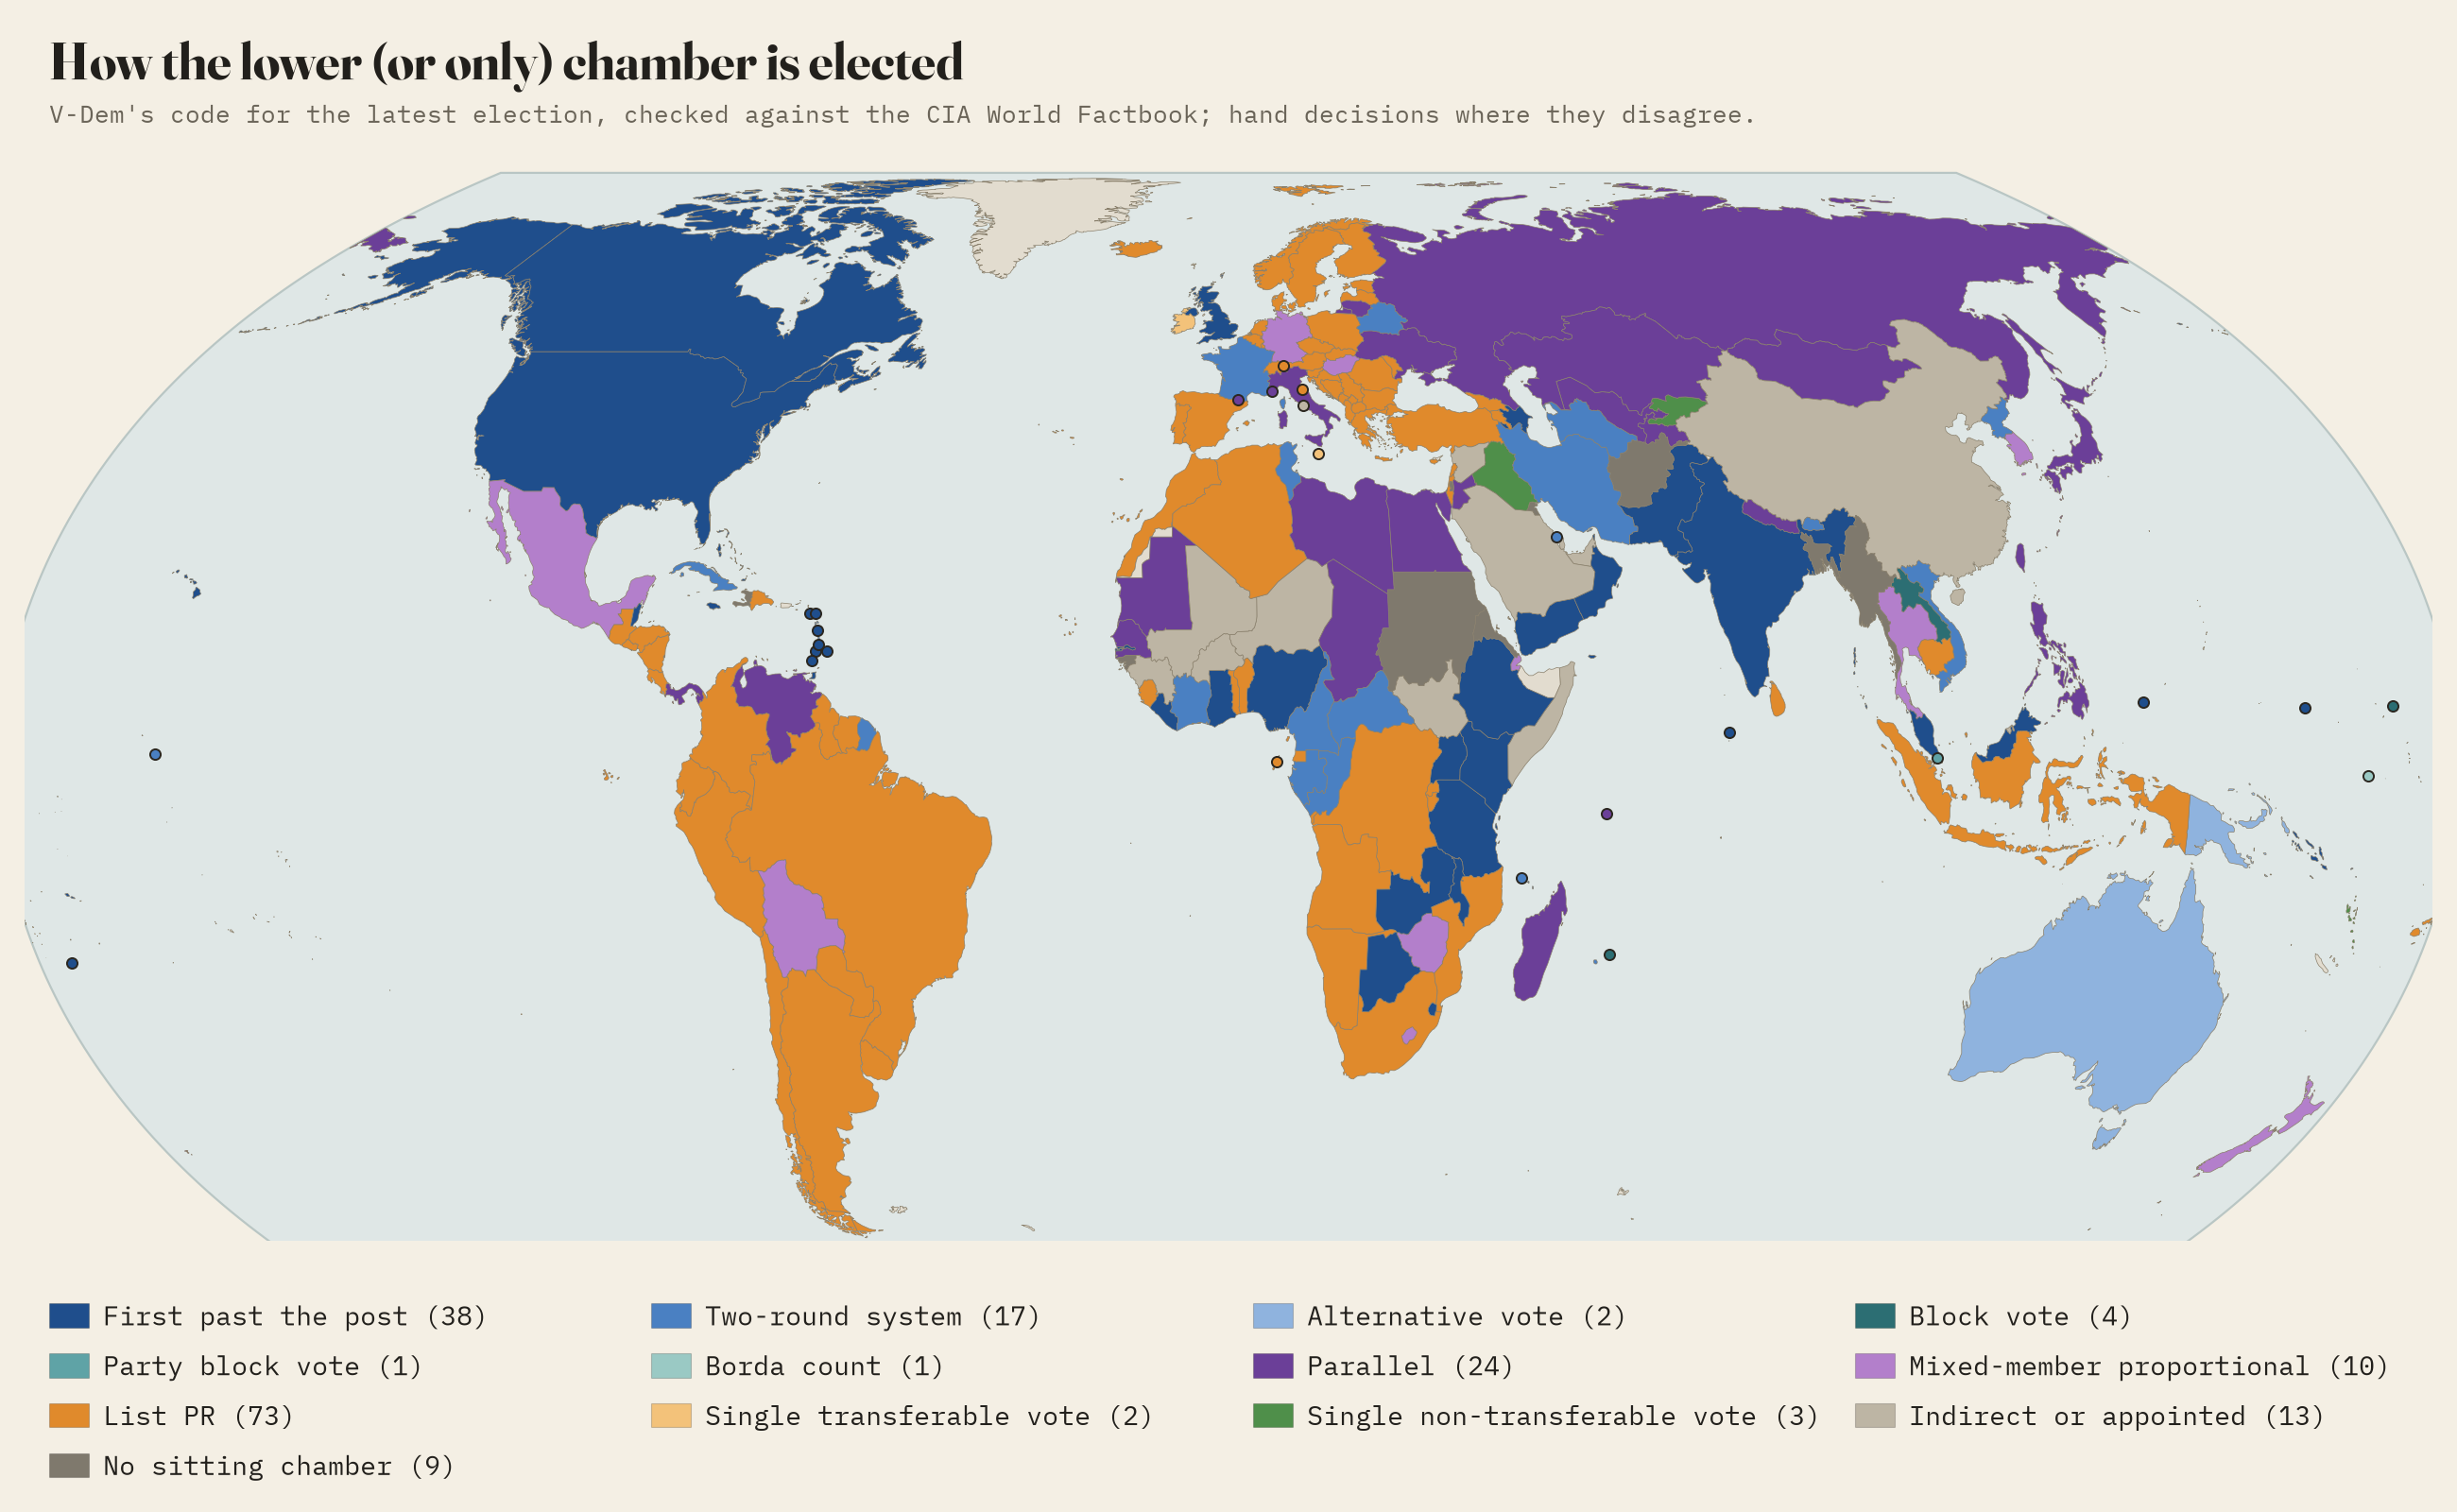
\includegraphics[width=\textwidth]{f_map_electoral.png}
\caption{Electoral system of the lower or only chamber.}\label{fig:elmap}\end{figure}

\subsection{Form and freedom}
V-Dem classes 33 countries as closed autocracies, 55 as electoral autocracies, 56 as electoral democracies and 31 as liberal democracies for 2025; 73\% of the world's people live in autocracies and 8\% in liberal democracies. Figure~\ref{fig:xreg} crosses the electoral system with regime type: 71\% of proportional, 44\% of mixed and 43\% of majoritarian countries are democracies, and 26\%, 25\% and 8\% respectively are liberal democracies. Among the 31 liberal democracies, 61\% use proportional representation, 26\% a mixed system and 13\% a majoritarian one.

Figure~\ref{fig:ldi} shows the Liberal Democracy Index by family. The 20 ceremonial monarchies scored by V-Dem have the highest mean (0.64, against 0.50 for parliamentary republics); 10 of them are liberal democracies, and the three highest-scoring countries on V-Dem's index are Denmark, Sweden and Norway. Cambodia, Papua New Guinea and Thailand are ceremonial monarchies classed as autocracies. Where the monarch rules, scores are low: the mean is 0.18 for ruling and 0.09 for absolute monarchies. 78\% of premier-presidential countries are democracies against 11\% of president-parliamentary ones; among presidential republics the share is 55\%, among parliamentary republics 69\%. These contrasts echo long-standing arguments about presidentialism \citep{linz,cheibub} and semi-presidential subtypes \citep{elgie2011}, but they are bivariate and descriptive: region, colonial inheritance, wealth and history shape both institutions and democracy, and in authoritarian states constitutions often describe the form rather than the reality of power.

\begin{figure}[tbp]\centering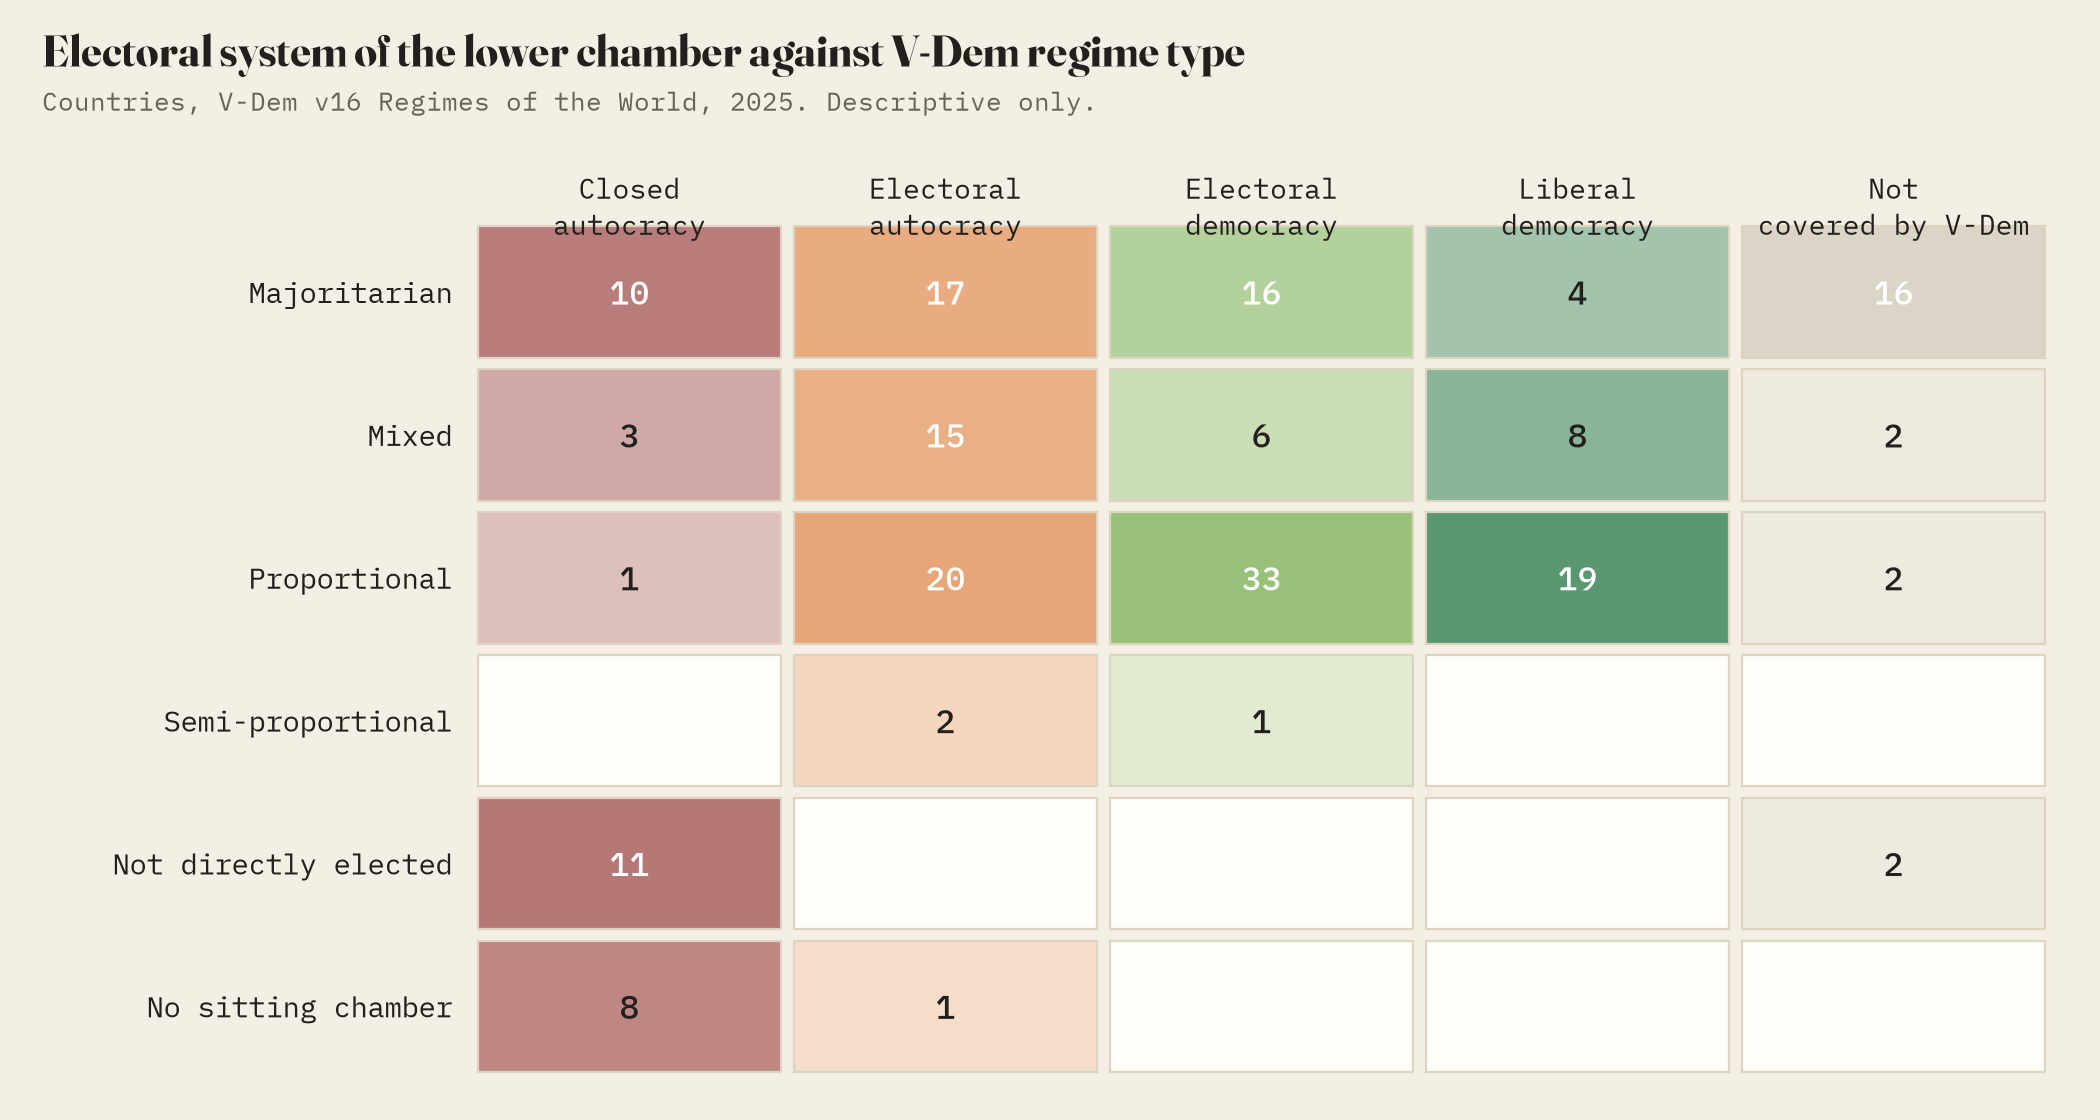
\includegraphics[width=.9\textwidth]{f_elec_regime.png}
\caption{Electoral system of the lower or only chamber against V-Dem Regimes of the World (2025), countries.}\label{fig:xreg}\end{figure}

\begin{figure}[tbp]\centering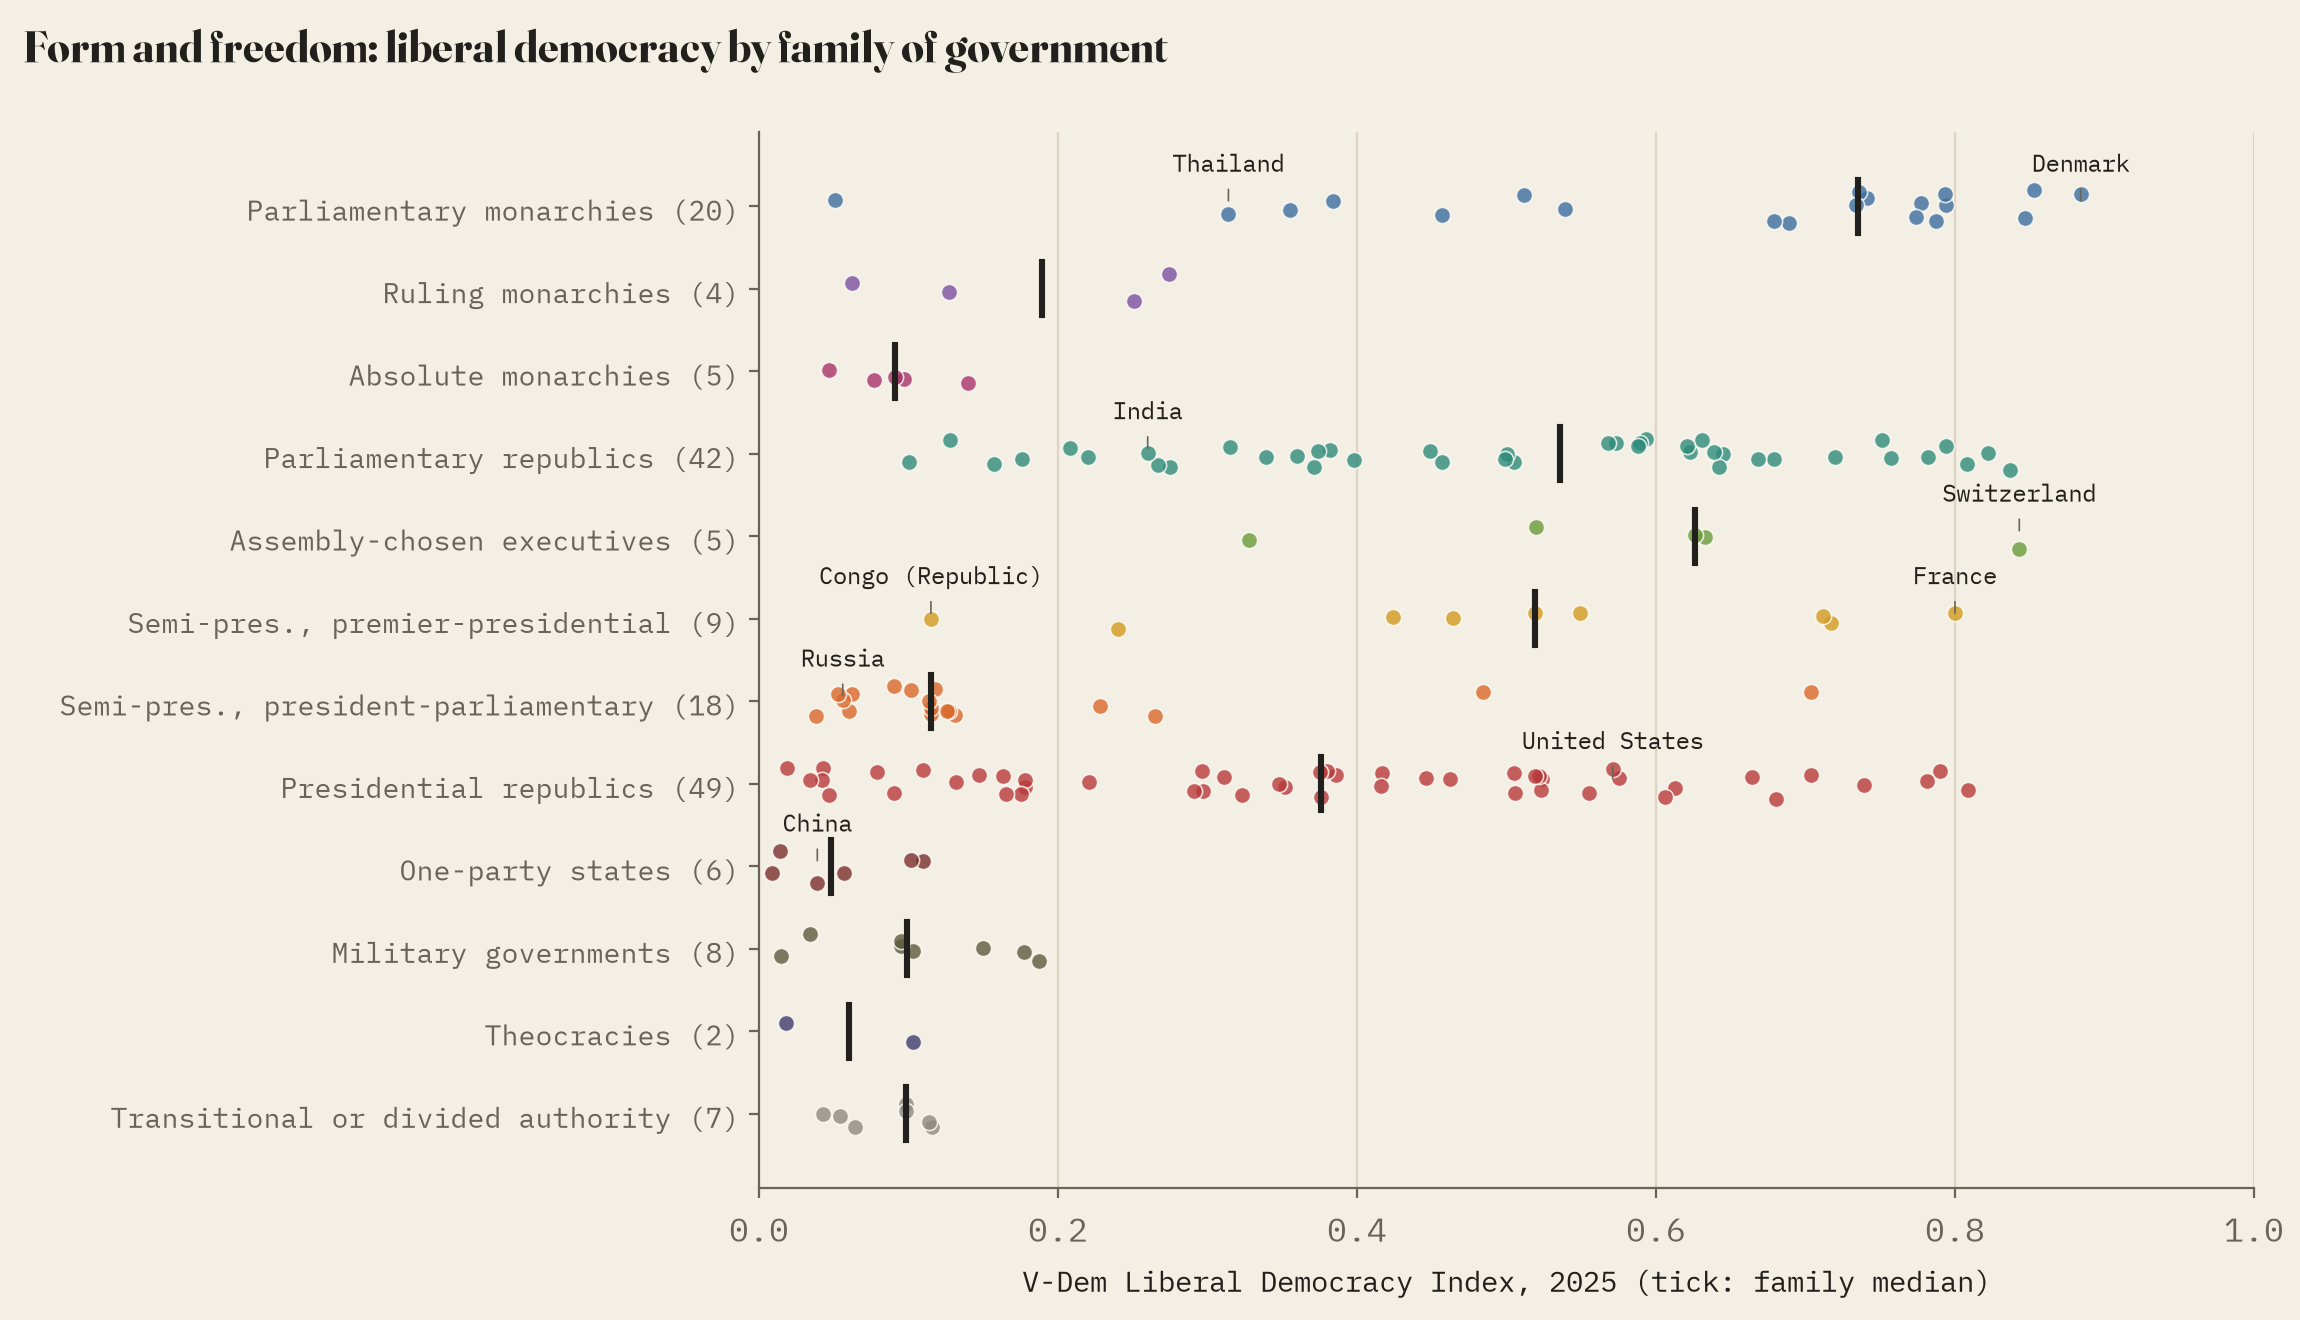
\includegraphics[width=\textwidth]{f_ldi.png}
\caption{V-Dem Liberal Democracy Index by family (2025); ticks mark medians.}\label{fig:ldi}\end{figure}

\subsection{Agreement between sources and hand decisions}
Where both sources speak to a field they agree in most cases (Table~\ref{tab:checks}). 51 country and field cells in 48 countries still disagree after the rules are applied. The largest group (14) are states the Factbook labels presidential that also have a prime minister whom V-Dem codes the president as able to dismiss; others are monarchies the Factbook calls parliamentary where V-Dem codes a ruling monarch (Jordan, Morocco) and military regimes the Factbook lists under their constitutional label. 83 hand decisions in 60 countries (66 rated high confidence, 17 medium) settle the remaining hard cases, among them the United Kingdom's asymmetric devolution, France's constitutional premier-presidentialism, Switzerland's directorial executive, Iran's Supreme Leader, Bosnia's federal structure and ethnic presidency, Lebanon's confessional power sharing, the Holy See, Andorra's co-princes, Malaysia's elective monarchy, the United Arab Emirates as a federation of absolute monarchies, and the transitional or military governments of Libya, Myanmar, Afghanistan, Sudan and Haiti (Table~\ref{tab:hard}). Every decision, with its reason and citation, is in the released data.

\begin{table}[tbp]\centering\small\caption{Agreement between V-Dem and the Factbook, countries per field. Other: not applicable (no elected chamber), derived from another field, or coded by hand only.}\label{tab:checks}\begin{tabular}{lrrrrr}\toprule Field & Agree & Disagree & One source & Hand decision & Other\\\midrule
Head of state & 166 & 5 & 17 & 9 & \\
Office filled by &  &  &  & 14 & 183\\
Executive & 144 & 30 &  & 23 & \\
HoS and HoG & 164 & 10 & 23 &  & \\
Territory &  &  & 181 & 16 & \\
Chambers & 164 & 4 & 25 & 4 & \\
Electoral system & 149 & 2 & 16 & 13 & 17\\
Power sharing &  &  &  & 4 & 193\\
\bottomrule\end{tabular}\end{table}

\begin{table}[tbp]\centering\footnotesize\caption{Classification of the hardest cases, with the hand decisions that set them (identifiers as in data/hand\_decisions.csv; ``rule'' where the sources agree and no decision was needed).}\label{tab:hard}\begin{tabular}{lp{8.2cm}p{3.2cm}}\toprule Country & Classification & Decisions\\\midrule
United Kingdom & \raggedright Ceremonial monarchy; Parliamentary; Regionalised; FPTP & H01\\
France & \raggedright Republic; Semi-pres. (premier-pres.); Unitary; Two-round & H11\\
Switzerland & \raggedright Republic; Directorial; Federal; List PR & H13 H14\\
Iran & \raggedright Republic; Theocratic; Unitary; Two-round & H16 H17\\
China & \raggedright Republic; One-party state; Unitary, auton. regions; Indirect/appointed & nan\\
Russia & \raggedright Republic; Semi-pres. (pres.-parl.); Federal; Parallel & nan\\
Bosnia and Herzegovina & \raggedright Republic; Parliamentary; Federal; List PR; ethnic power sharing & H05 H06 H07\\
Lebanon & \raggedright Republic; Parliamentary; Unitary; List PR; confessional power sharing & H08\\
Holy See (Vatican City) & \raggedright Absolute monarchy; Theocratic; Unitary; Indirect/appointed & H21 H22 H23\\
Andorra & \raggedright Ceremonial monarchy; Parliamentary; Unitary; Parallel & H24 H25 H26\\
Malaysia & \raggedright Ceremonial monarchy; Parliamentary; Federal; FPTP & H27\\
United Arab Emirates & \raggedright Absolute monarchy; Royal (absolute); Federal; Indirect/appointed & H29 H30 H31\\
Libya & \raggedright Republic; Transitional; Unitary; Parallel & H32 H33\\
Myanmar & \raggedright Republic; Military government; Unitary; None sitting & H34\\
Afghanistan & \raggedright Theocratic emirate; Theocratic; Unitary; None sitting & H18 H19 H20\\
Sudan & \raggedright Republic; Military government; Unitary; None sitting & H35 H36\\
Haiti & \raggedright Republic; Transitional; Unitary; None sitting & H37 H38\\
\bottomrule\end{tabular}\end{table}

\section{Discussion}
Moving from a binary to eight fields changes what a world map of government shows. At family level the map is dominated by two large blocks, presidential republics in the Americas and Africa and parliamentary systems in Europe, South Asia and the old Commonwealth, with a belt of president-parliamentary systems across North Africa and the former Soviet Union and a small but populous set of one-party states in East Asia. At the level of exact systems, institutional design turns out to be highly individual: two in five countries have a combination nobody else uses, among them China, Indonesia and Russia. Shared systems cluster regionally, which is what one would expect from diffusion of constitutional models, from post-communist Europe's list-PR parliamentary republics to Latin America's presidential list-PR republics and the Caribbean realms' Westminster template.

The classification separates form from quality on purpose. That France and the Republic of the Congo share an exact constitutional form, or that ceremonial monarchy co-exists with both the highest and some of the lowest liberal democracy scores, are reminders that institutional labels are not regime outcomes. The descriptive associations reported here, between proportional representation, premier-presidential semi-presidentialism and parliamentary monarchy on one side and democracy on the other, are consistent with comparative research but should not be read causally.

\section{Limitations}
First, every typology flattens: degrees of federalism, of presidential power and of proportionality are continuous, and the thresholds used (for example V-Dem's in-practice indicator at 0.5 for the semi-presidential subtype) decide borderline cases. Second, the two sources differ in kind: V-Dem codes practice through expert surveys, with uncertainty; the Factbook describes the constitution and sometimes lags behind changes. Third, the electoral system is that of the latest coded election and may since have been reformed. Fourth, V-Dem does not cover 22 small states, whose fields rest on the Factbook and hand decisions. Fifth, the reference date is the start of 2026, and some countries (Guinea, Myanmar, Syria) were changing as it passed. Sixth, power sharing is coded narrowly and reserved seats for minorities are not coded. Finally, Wikidata and Wikipedia, natural third sources, could not be used in this version.

\section{Conclusion}
The world's 197 states fall into 12 families of government but 112 exact systems, and 80 countries, holding 42\% of humanity, share their system with nobody. Classifying form and quality separately, from cross-checked open sources with every judgement documented, gives a map of how countries are put together that sits beside, rather than replaces, maps of how democratic they are.

\section*{Data and code availability}
The interactive map is at \url{https://maps.tristanhotham.com/government-types/}. Data and code are at \url{https://github.com/Tristan-Hotham/government-types} and archived with this paper at https://doi.org/10.5281/zenodo.23863540. Because the data include V-Dem values, the derived data, text and figures are released under CC BY-SA 4.0; code under the MIT licence. The Factbook is public domain, World Bank data CC BY 4.0 and Natural Earth public domain.

\section*{AI statement}
I wrote the text, with drafting and editing assistance from Claude (Anthropic), which also helped prepare the analysis code. I reviewed and checked all text and results.

\begin{thebibliography}{20}
\bibitem[Cheibub(2007)]{cheibub} Cheibub, J. A. (2007) \emph{Presidentialism, Parliamentarism, and Democracy}. Cambridge: Cambridge University Press.
\bibitem[CIA(2026)]{factbook} Central Intelligence Agency (2026) \emph{The World Factbook}, 2026 and December 2024 editions. Public domain. As JSON: \url{https://github.com/factbook/factbook.json}
\bibitem[Coppedge et al.(2026)]{vdem} Coppedge, M., Gerring, J., Knutsen, C. H., Lindberg, S. I., Teorell, J. et al. (2026) V-Dem Country-Year Dataset v16. Varieties of Democracy (V-Dem) Project. \url{https://doi.org/10.23696/vdemds26}
\bibitem[Duverger(1980)]{duverger} Duverger, M. (1980) A new political system model: semi-presidential government. \emph{European Journal of Political Research} 8(2), 165 to 187.
\bibitem[Elgie(2011)]{elgie2011} Elgie, R. (2011) \emph{Semi-Presidentialism: Sub-Types and Democratic Performance}. Oxford: Oxford University Press.
\bibitem[Lijphart(2012)]{lijphart} Lijphart, A. (2012) \emph{Patterns of Democracy: Government Forms and Performance in Thirty-Six Countries}. 2nd edn. New Haven: Yale University Press.
\bibitem[Linz(1990)]{linz} Linz, J. J. (1990) The perils of presidentialism. \emph{Journal of Democracy} 1(1), 51 to 69.
\bibitem[Lührmann et al.(2018)]{row} Lührmann, A., Tannenberg, M. and Lindberg, S. I. (2018) Regimes of the World (RoW): opening new avenues for the comparative study of political regimes. \emph{Politics and Governance} 6(1), 60 to 77.
\bibitem[Maerz et al.(2026)]{vdemdata} Maerz, S. F., Edgell, A. B., Hellmeier, S., Ilchenko, N. and Fox, L. (2026) vdemdata: an R package to load, explore and work with the most recent V-Dem dataset, version 16.0. \url{https://github.com/vdeminstitute/vdemdata}
\bibitem[Natural Earth(2026)]{naturalearth} Natural Earth (2026) Admin 0 countries, 1:10m and 1:50m. Public domain. \url{https://www.naturalearthdata.com/}
\bibitem[Reynolds et al.(2005)]{reynolds} Reynolds, A., Reilly, B. and Ellis, A. (2005) \emph{Electoral System Design: The New International IDEA Handbook}. Stockholm: International IDEA.
\bibitem[Shugart and Carey(1992)]{shugartcarey} Shugart, M. S. and Carey, J. M. (1992) \emph{Presidents and Assemblies: Constitutional Design and Electoral Dynamics}. Cambridge: Cambridge University Press.
\bibitem[World Bank(2026)]{wb} World Bank (2026) World Development Indicators: population, total (SP.POP.TOTL). CC BY 4.0. Via \url{https://github.com/datasets/population}
\end{thebibliography}

\clearpage
\appendix
\section{All 197 countries}
{\tiny\setlength{\tabcolsep}{2.5pt}\renewcommand{\arraystretch}{0.92}\begin{longtable}{p{2.9cm}lp{2.9cm}p{2.4cm}lp{1.9cm}p{2.0cm}}\caption{Classification of every country. Family codes: PM Parliamentary monarchies; RM Ruling monarchies; AM Absolute monarchies; PR Parliamentary republics; AE Assembly-chosen executives; SP Semi-presidential, premier-presidential; SR Semi-presidential, president-parliamentary; PS Presidential republics; OP One-party states; MI Military governments; TH Theocracies; TR Transitional or divided authority.}\\\toprule Country & Fam. & Executive & Territory & Chambers & Electoral system & V-Dem regime\\\midrule\endfirsthead\toprule Country & Fam. & Executive & Territory & Chambers & Electoral system & V-Dem regime\\\midrule\endhead
Afghanistan & TH & Theocratic & Unitary & None sitting & None sitting & Closed autocracy\\
Albania & PR & Parliamentary & Unitary & Unicameral & List PR & Electoral autocracy\\
Algeria & SR & Semi-pres. (pres.-parl.) & Unitary & Bicameral & List PR & Electoral autocracy\\
Andorra & PM & Parliamentary & Unitary & Unicameral & Parallel & not in V-Dem\\
Angola & PS & Presidential & Unitary & Unicameral & List PR & Electoral autocracy\\
Antigua and Barbuda & PM & Parliamentary & Unitary & Bicameral & FPTP & not in V-Dem\\
Argentina & PS & Presidential & Federal & Bicameral & List PR & Electoral democracy\\
Armenia & PR & Parliamentary & Unitary & Unicameral & List PR & Electoral democracy\\
Australia & PM & Parliamentary & Federal & Bicameral & Alternative vote & Liberal democracy\\
Austria & PR & Parliamentary & Federal & Bicameral & List PR & Liberal democracy\\
Azerbaijan & SR & Semi-pres. (pres.-parl.) & Unitary, auton. regions & Unicameral & FPTP & Electoral autocracy\\
Bahamas & PM & Parliamentary & Unitary & Bicameral & FPTP & not in V-Dem\\
Bahrain & RM & Dualist & Unitary & Bicameral & Two-round & Closed autocracy\\
Bangladesh & TR & Transitional & Unitary & None sitting & None sitting & Closed autocracy\\
Barbados & PR & Parliamentary & Unitary & Bicameral & FPTP & Liberal democracy\\
Belarus & SR & Semi-pres. (pres.-parl.) & Unitary & Bicameral & Two-round & Closed autocracy\\
Belgium & PM & Parliamentary & Federal & Bicameral & List PR & Liberal democracy\\
Belize & PM & Parliamentary & Unitary & Bicameral & FPTP & not in V-Dem\\
Benin & PS & Presidential & Unitary & Unicameral & List PR & Electoral autocracy\\
Bhutan & PM & Parliamentary & Unitary & Bicameral & Two-round & Electoral democracy\\
Bolivia & PS & Presidential & Unitary & Bicameral & MMP & Electoral democracy\\
Bosnia and Herzegovina & PR & Parliamentary & Federal & Bicameral & List PR & Electoral autocracy\\
Botswana & AE & Parl., exec. president & Unitary & Unicameral & FPTP & Electoral democracy\\
Brazil & PS & Presidential & Federal & Bicameral & List PR & Electoral democracy\\
Brunei & AM & Royal (absolute) & Unitary & Unicameral & Indirect/appointed & not in V-Dem\\
Bulgaria & PR & Parliamentary & Unitary & Unicameral & List PR & Electoral democracy\\
Burkina Faso & MI & Military government & Unitary & Unicameral & Indirect/appointed & Closed autocracy\\
Burundi & SR & Semi-pres. (pres.-parl.) & Unitary & Bicameral & List PR & Electoral autocracy\\
Cabo Verde & PR & Parliamentary & Unitary & Unicameral & List PR & Electoral democracy\\
Cambodia & PM & Parliamentary & Unitary & Bicameral & List PR & Electoral autocracy\\
Cameroon & SR & Semi-pres. (pres.-parl.) & Unitary & Bicameral & Two-round & Electoral autocracy\\
Canada & PM & Parliamentary & Federal & Bicameral & FPTP & Electoral democracy\\
Central African Republic & SR & Semi-pres. (pres.-parl.) & Unitary & Unicameral & Two-round & Electoral autocracy\\
Chad & SR & Semi-pres. (pres.-parl.) & Unitary & Bicameral & Parallel & Electoral autocracy\\
Chile & PS & Presidential & Unitary & Bicameral & List PR & Liberal democracy\\
China & OP & One-party state & Unitary, auton. regions & Unicameral & Indirect/appointed & Closed autocracy\\
Colombia & PS & Presidential & Unitary & Bicameral & List PR & Electoral democracy\\
Comoros & PS & Presidential & Federal & Unicameral & Two-round & Electoral autocracy\\
Congo (Republic) & SP & Semi-pres. (premier-pres.) & Unitary & Bicameral & Two-round & Electoral autocracy\\
Costa Rica & PS & Presidential & Unitary & Unicameral & List PR & Liberal democracy\\
Croatia & PR & Parliamentary & Unitary & Unicameral & List PR & Electoral democracy\\
Cuba & OP & One-party state & Unitary & Unicameral & Two-round & Closed autocracy\\
Cyprus & PS & Presidential & Unitary & Unicameral & List PR & Liberal democracy\\
Czechia & PR & Parliamentary & Unitary & Bicameral & List PR & Liberal democracy\\
Côte d'Ivoire & SR & Semi-pres. (pres.-parl.) & Unitary & Bicameral & Two-round & Electoral autocracy\\
DR Congo & SR & Semi-pres. (pres.-parl.) & Unitary & Bicameral & List PR & Electoral autocracy\\
Denmark & PM & Parliamentary & Unitary, auton. regions & Unicameral & List PR & Liberal democracy\\
Djibouti & SR & Semi-pres. (pres.-parl.) & Unitary & Unicameral & MMP & Electoral autocracy\\
Dominica & PR & Parliamentary & Unitary & Unicameral & FPTP & not in V-Dem\\
Dominican Republic & PS & Presidential & Unitary & Bicameral & List PR & Electoral democracy\\
Ecuador & PS & Presidential & Unitary & Unicameral & List PR & Electoral democracy\\
Egypt & SR & Semi-pres. (pres.-parl.) & Unitary & Bicameral & Parallel & Electoral autocracy\\
El Salvador & PS & Presidential & Unitary & Unicameral & List PR & Electoral autocracy\\
Equatorial Guinea & PS & Presidential & Unitary & Bicameral & List PR & Electoral autocracy\\
Eritrea & OP & One-party state & Unitary & None sitting & None sitting & Closed autocracy\\
Estonia & PR & Parliamentary & Unitary & Unicameral & List PR & Liberal democracy\\
Eswatini & AM & Royal (absolute) & Unitary & Bicameral & FPTP & Closed autocracy\\
Ethiopia & PR & Parliamentary & Federal & Bicameral & FPTP & Electoral autocracy\\
Fiji & PR & Parliamentary & Unitary & Unicameral & List PR & Electoral democracy\\
Finland & PR & Parliamentary & Unitary, auton. regions & Unicameral & List PR & Liberal democracy\\
France & SP & Semi-pres. (premier-pres.) & Unitary & Bicameral & Two-round & Liberal democracy\\
Gabon & PS & Presidential & Unitary & Bicameral & Two-round & Electoral autocracy\\
Gambia & PS & Presidential & Unitary & Unicameral & FPTP & Electoral democracy\\
Georgia & PR & Parliamentary & Unitary, auton. regions & Unicameral & List PR & Electoral autocracy\\
Germany & PR & Parliamentary & Federal & Bicameral & MMP & Liberal democracy\\
Ghana & PS & Presidential & Unitary & Unicameral & FPTP & Electoral democracy\\
Greece & PR & Parliamentary & Unitary, auton. regions & Unicameral & List PR & Electoral democracy\\
Grenada & PM & Parliamentary & Unitary & Bicameral & FPTP & not in V-Dem\\
Guatemala & PS & Presidential & Unitary & Unicameral & List PR & Electoral democracy\\
Guinea & MI & Military government & Unitary & Unicameral & Indirect/appointed & Closed autocracy\\
Guinea-Bissau & MI & Military government & Unitary & None sitting & None sitting & Closed autocracy\\
Guyana & AE & Parl., exec. president & Unitary & Unicameral & List PR & Electoral democracy\\
Haiti & TR & Transitional & Unitary & None sitting & None sitting & Closed autocracy\\
Holy See (Vatican City) & TH & Theocratic & Unitary & Unicameral & Indirect/appointed & not in V-Dem\\
Honduras & PS & Presidential & Unitary & Unicameral & List PR & Electoral democracy\\
Hungary & PR & Parliamentary & Unitary & Unicameral & MMP & Electoral autocracy\\
Iceland & PR & Parliamentary & Unitary & Unicameral & List PR & Liberal democracy\\
India & PR & Parliamentary & Federal & Bicameral & FPTP & Electoral autocracy\\
Indonesia & PS & Presidential & Unitary, auton. regions & Bicameral & List PR & Electoral autocracy\\
Iran & TH & Theocratic & Unitary & Unicameral & Two-round & Electoral autocracy\\
Iraq & PR & Parliamentary & Federal & Unicameral & SNTV & Electoral autocracy\\
Ireland & PR & Parliamentary & Unitary & Bicameral & STV & Liberal democracy\\
Israel & PR & Parliamentary & Unitary & Unicameral & List PR & Electoral democracy\\
Italy & PR & Parliamentary & Regionalised & Bicameral & Parallel & Liberal democracy\\
Jamaica & PM & Parliamentary & Unitary & Bicameral & FPTP & Electoral democracy\\
Japan & PM & Parliamentary & Unitary & Bicameral & Parallel & Liberal democracy\\
Jordan & RM & Dualist & Unitary & Bicameral & Parallel & Closed autocracy\\
Kazakhstan & SR & Semi-pres. (pres.-parl.) & Unitary & Bicameral & Parallel & Electoral autocracy\\
Kenya & PS & Presidential & Unitary & Bicameral & FPTP & Electoral democracy\\
Kiribati & PS & Presidential & Unitary & Unicameral & Two-round & not in V-Dem\\
Kosovo & PR & Parliamentary & Unitary & Unicameral & List PR & Electoral democracy\\
Kuwait & RM & Dualist & Unitary & None sitting & None sitting & Closed autocracy\\
Kyrgyzstan & PS & Presidential & Unitary & Unicameral & SNTV & Electoral autocracy\\
Laos & OP & One-party state & Unitary & Unicameral & Block vote & Closed autocracy\\
Latvia & PR & Parliamentary & Unitary & Unicameral & List PR & Liberal democracy\\
Lebanon & PR & Parliamentary & Unitary & Unicameral & List PR & Electoral autocracy\\
Lesotho & PM & Parliamentary & Unitary & Bicameral & MMP & Electoral democracy\\
Liberia & PS & Presidential & Unitary & Bicameral & FPTP & Electoral democracy\\
Libya & TR & Transitional & Unitary & Unicameral & Parallel & Closed autocracy\\
Liechtenstein & RM & Dualist & Unitary & Unicameral & List PR & not in V-Dem\\
Lithuania & SP & Semi-pres. (premier-pres.) & Unitary & Unicameral & Parallel & Liberal democracy\\
Luxembourg & PM & Parliamentary & Unitary & Unicameral & List PR & Liberal democracy\\
Madagascar & MI & Military government & Unitary & Bicameral & Parallel & Electoral autocracy\\
Malawi & PS & Presidential & Unitary & Unicameral & FPTP & Electoral democracy\\
Malaysia & PM & Parliamentary & Federal & Bicameral & FPTP & Electoral democracy\\
Maldives & PS & Presidential & Unitary & Unicameral & FPTP & Electoral democracy\\
Mali & MI & Military government & Unitary & Unicameral & Indirect/appointed & Closed autocracy\\
Malta & PR & Parliamentary & Unitary & Unicameral & STV & Electoral democracy\\
Marshall Islands & PS & Presidential & Unitary & Unicameral & Block vote & not in V-Dem\\
Mauritania & SR & Semi-pres. (pres.-parl.) & Unitary & Unicameral & Parallel & Electoral autocracy\\
Mauritius & PR & Parliamentary & Unitary, auton. regions & Unicameral & Block vote & Electoral democracy\\
Mexico & PS & Presidential & Federal & Bicameral & MMP & Electoral autocracy\\
Micronesia & AE & Parl., exec. president & Federal & Unicameral & FPTP & not in V-Dem\\
Moldova & PR & Parliamentary & Unitary, auton. regions & Unicameral & List PR & Electoral democracy\\
Monaco & RM & Dualist & Unitary & Unicameral & Parallel & not in V-Dem\\
Mongolia & SP & Semi-pres. (premier-pres.) & Unitary & Unicameral & Parallel & Electoral democracy\\
Montenegro & PR & Parliamentary & Unitary & Unicameral & List PR & Electoral democracy\\
Morocco & RM & Dualist & Unitary & Bicameral & List PR & Closed autocracy\\
Mozambique & PS & Presidential & Unitary & Unicameral & List PR & Electoral autocracy\\
Myanmar & MI & Military government & Unitary & None sitting & None sitting & Closed autocracy\\
Namibia & PS & Presidential & Unitary & Bicameral & List PR & Electoral democracy\\
Nauru & AE & Parl., exec. president & Unitary & Unicameral & Borda count & not in V-Dem\\
Nepal & PR & Parliamentary & Federal & Bicameral & Parallel & Electoral democracy\\
Netherlands & PM & Parliamentary & Unitary, auton. regions & Bicameral & List PR & Liberal democracy\\
New Zealand & PM & Parliamentary & Unitary & Unicameral & MMP & Liberal democracy\\
Nicaragua & PS & Presidential & Unitary, auton. regions & Unicameral & List PR & Electoral autocracy\\
Niger & MI & Military government & Unitary & Unicameral & Indirect/appointed & Closed autocracy\\
Nigeria & PS & Presidential & Federal & Bicameral & FPTP & Electoral democracy\\
North Korea & OP & One-party state & Unitary & Unicameral & Two-round & Closed autocracy\\
North Macedonia & PR & Parliamentary & Unitary & Unicameral & List PR & Electoral democracy\\
Norway & PM & Parliamentary & Unitary & Unicameral & List PR & Liberal democracy\\
Oman & AM & Royal (absolute) & Unitary & Bicameral & FPTP & Closed autocracy\\
Pakistan & PR & Parliamentary & Federal & Bicameral & FPTP & Electoral autocracy\\
Palau & PS & Presidential & Unitary & Bicameral & FPTP & not in V-Dem\\
Palestine & TR & Transitional & Unitary & None sitting & None sitting & Electoral autocracy\\
Panama & PS & Presidential & Unitary & Unicameral & Parallel & Electoral democracy\\
Papua New Guinea & PM & Parliamentary & Unitary, auton. regions & Unicameral & Alternative vote & Electoral autocracy\\
Paraguay & PS & Presidential & Unitary & Bicameral & List PR & Electoral democracy\\
Peru & PS & Presidential & Unitary & Unicameral & List PR & Electoral democracy\\
Philippines & PS & Presidential & Unitary, auton. regions & Bicameral & Parallel & Electoral autocracy\\
Poland & PR & Parliamentary & Unitary & Bicameral & List PR & Electoral democracy\\
Portugal & SP & Semi-pres. (premier-pres.) & Unitary, auton. regions & Unicameral & List PR & Electoral democracy\\
Qatar & AM & Royal (absolute) & Unitary & Unicameral & Indirect/appointed & Closed autocracy\\
Romania & SP & Semi-pres. (premier-pres.) & Unitary & Bicameral & List PR & Electoral democracy\\
Russia & SR & Semi-pres. (pres.-parl.) & Federal & Bicameral & Parallel & Electoral autocracy\\
Rwanda & SR & Semi-pres. (pres.-parl.) & Unitary & Bicameral & List PR & Electoral autocracy\\
Saint Kitts and Nevis & PM & Parliamentary & Federal & Unicameral & FPTP & not in V-Dem\\
Saint Lucia & PM & Parliamentary & Unitary & Bicameral & FPTP & not in V-Dem\\
Saint Vincent and the Grenadines & PM & Parliamentary & Unitary & Unicameral & FPTP & not in V-Dem\\
Samoa & PR & Parliamentary & Unitary & Unicameral & FPTP & not in V-Dem\\
San Marino & PR & Parliamentary & Unitary & Unicameral & List PR & not in V-Dem\\
Saudi Arabia & AM & Royal (absolute) & Unitary & Unicameral & Indirect/appointed & Closed autocracy\\
Senegal & SR & Semi-pres. (pres.-parl.) & Unitary & Unicameral & Parallel & Electoral democracy\\
Serbia & PR & Parliamentary & Unitary, auton. regions & Unicameral & List PR & Electoral autocracy\\
Seychelles & PS & Presidential & Unitary & Unicameral & Parallel & Liberal democracy\\
Sierra Leone & PS & Presidential & Unitary & Unicameral & List PR & Electoral autocracy\\
Singapore & PR & Parliamentary & Unitary & Unicameral & Party block vote & Electoral autocracy\\
Slovakia & PR & Parliamentary & Unitary & Unicameral & List PR & Electoral democracy\\
Slovenia & PR & Parliamentary & Unitary & Bicameral & List PR & Electoral democracy\\
Solomon Islands & PM & Parliamentary & Unitary & Unicameral & FPTP & Electoral democracy\\
Somalia & PR & Parliamentary & Federal & Bicameral & Indirect/appointed & Closed autocracy\\
South Africa & AE & Parl., exec. president & Unitary & Bicameral & List PR & Electoral democracy\\
South Korea & PS & Presidential & Unitary & Unicameral & MMP & Liberal democracy\\
South Sudan & TR & Transitional & Unitary & Bicameral & Indirect/appointed & Closed autocracy\\
Spain & PM & Parliamentary & Regionalised & Bicameral & List PR & Liberal democracy\\
Sri Lanka & PS & Presidential & Unitary & Unicameral & List PR & Electoral democracy\\
Sudan & MI & Military government & Unitary & None sitting & None sitting & Closed autocracy\\
Suriname & AE & Parl., exec. president & Unitary & Unicameral & List PR & Electoral democracy\\
Sweden & PM & Parliamentary & Unitary & Unicameral & List PR & Liberal democracy\\
Switzerland & AE & Directorial & Federal & Bicameral & List PR & Liberal democracy\\
Syria & TR & Transitional & Unitary & Unicameral & Indirect/appointed & Closed autocracy\\
São Tomé and Príncipe & SP & Semi-pres. (premier-pres.) & Unitary, auton. regions & Unicameral & List PR & Electoral democracy\\
Taiwan & SR & Semi-pres. (pres.-parl.) & Unitary & Unicameral & Parallel & Liberal democracy\\
Tajikistan & PS & Presidential & Unitary, auton. regions & Bicameral & Parallel & Electoral autocracy\\
Tanzania & PS & Presidential & Unitary, auton. regions & Unicameral & FPTP & Electoral autocracy\\
Thailand & PM & Parliamentary & Unitary & Bicameral & MMP & Electoral autocracy\\
Timor-Leste & SP & Semi-pres. (premier-pres.) & Unitary & Unicameral & List PR & Electoral democracy\\
Togo & PR & Parliamentary & Unitary & Bicameral & List PR & Electoral autocracy\\
Tonga & RM & Dualist & Unitary & Unicameral & FPTP & not in V-Dem\\
Trinidad and Tobago & PR & Parliamentary & Unitary, auton. regions & Bicameral & FPTP & Liberal democracy\\
Tunisia & SR & Semi-pres. (pres.-parl.) & Unitary & Bicameral & Two-round & Electoral autocracy\\
Turkey & PS & Presidential & Unitary & Unicameral & List PR & Electoral autocracy\\
Turkmenistan & PS & Presidential & Unitary & Unicameral & Two-round & Closed autocracy\\
Tuvalu & PM & Parliamentary & Unitary & Unicameral & Block vote & not in V-Dem\\
Uganda & PS & Presidential & Unitary & Unicameral & FPTP & Electoral autocracy\\
Ukraine & SP & Semi-pres. (premier-pres.) & Unitary, auton. regions & Unicameral & Parallel & Electoral autocracy\\
United Arab Emirates & AM & Royal (absolute) & Federal & Unicameral & Indirect/appointed & Closed autocracy\\
United Kingdom & PM & Parliamentary & Regionalised & Bicameral & FPTP & Electoral democracy\\
United States & PS & Presidential & Federal & Bicameral & FPTP & Electoral democracy\\
Uruguay & PS & Presidential & Unitary & Bicameral & List PR & Liberal democracy\\
Uzbekistan & PS & Presidential & Unitary, auton. regions & Bicameral & Parallel & Closed autocracy\\
Vanuatu & PR & Parliamentary & Unitary & Unicameral & SNTV & Electoral democracy\\
Venezuela & PS & Presidential & Federal & Unicameral & Parallel & Electoral autocracy\\
Vietnam & OP & One-party state & Unitary & Unicameral & Two-round & Closed autocracy\\
Yemen & TR & Transitional & Unitary & Bicameral & FPTP & Closed autocracy\\
Zambia & PS & Presidential & Unitary & Unicameral & FPTP & Electoral autocracy\\
Zimbabwe & PS & Presidential & Unitary & Bicameral & MMP & Electoral autocracy\\
\bottomrule\end{longtable}}
\end{document}
